\documentclass[borders=2pt]{standalone}

% Drawing
\usepackage{tikz}

% Define Color
\definecolor{g1}{rgb}{0.0, 1.0, 0.0}

% Tikz Library
\usetikzlibrary{angles, quotes, calc, decorations.markings, decorations.pathmorphing, intersections}

% Styles
\tikzset{every node/.style={align=center}}
\tikzset{arrow inside/.style = {postaction=decorate,decoration={markings,mark=at position .52 with \arrow{stealth}}}}
\tikzset{ray/.style={very thick, red}}
\tikzset{line/.style={thick, black}}
\tikzset{lined/.style={thick, black, dashed}}

\begin{document}
	
	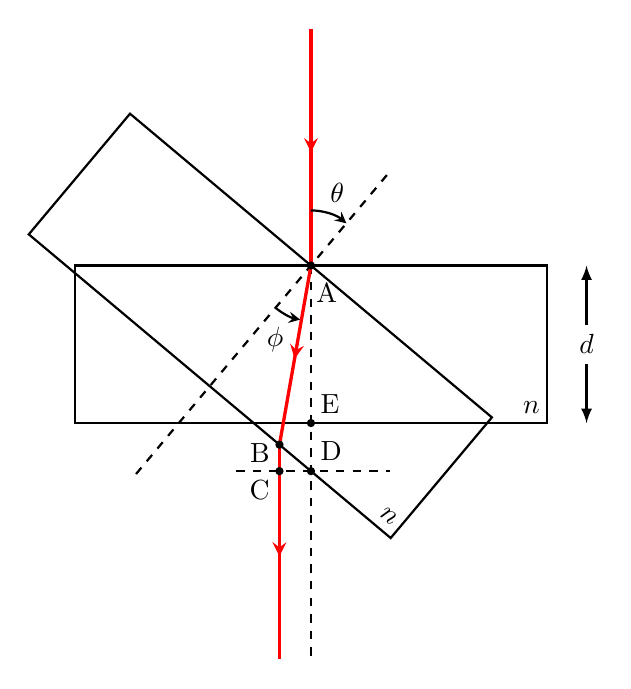
\begin{tikzpicture}
	
%		% Grid
%		\draw[dotted, black!30] (0,0) grid (10,10);
%		\foreach \i in {0,...,10}
%		{
%			\node at (-2ex,\i) {\i};
%			\node at (\i,-2ex) {\i};
%		}
		
		% Coordinates
		%% Rays
		\coordinate (A') at (5,9);
		\coordinate (A'') at (5,1);
		\coordinate (B) at (4.6,4);
		\coordinate (B') at (4.6,1);
		%% Rectangles
		\coordinate (a) at (2,6);
		\coordinate (b) at (8,4);
		%% Comptutated
		\coordinate (A) at ($(a)+(3,0)$);
		
		% Rays
		\draw[name path=ray1, ray, arrow inside] (A') -- (A);
		
		% Rectangles
		\draw[name path=rect, line] (a) rectangle (b);
		\draw[name path=rect_rot, line, rotate around = {-40:(A)}] (2,6) rectangle (8,4);
		
		% Dashed
		\draw[name path=dashed1, lined] (A) -- (A'');
		\draw[lined, rotate around={-40:(A)}] (5,7.5) coordinate (k) -- (5,2.5) coordinate (k');
		\draw[name path=dashed2, white] ($(B)+(0,-0.05)$) -- (B'); % white line for B intersection
		
		% Intersection For Points D, E, B
		\path [name intersections={of=dashed1 and rect_rot, by={rrd1, rrd2}}] ;
		\path [name intersections={of=dashed1 and rect, by={rd1, rd2}}] ;
		\path [name intersections={of=dashed2 and rect_rot, by={rrd2}}] ;
		
		% Refracted Rays
		\draw[ray, arrow inside] (A) -- (rrd2);
		\draw[name path = ray2, ray, arrow inside] (rrd2) -- (B');
		
		% Dashed
		\draw[lined, name path=dashed3] (rrd1) -- +(-1,0) -- +(1,0);
		
		% Intersection for Point C
		\path [name intersections={of=dashed3 and ray2, by={r2d3_1, r2rd3_2}}] ;
	
		% Angles
		\pic[draw, stealth-, line, "$\theta$", angle radius=0.7cm, angle eccentricity=1.4] {angle=k--A--A'};
		\pic[draw, -stealth, line, "$\phi$", angle radius=0.7cm, angle eccentricity=1.5] {angle=k'--A--B};
		
		% Arrows
		\node at (8.5,5) (S) {$d$};
		\draw[latex-, thick] (8.5,6) -- (S);
		\draw[latex-, thick] (8.5,4) -- (S);
		
		% Nodes
		\fill (A) circle (1.5pt) node [shift={(0.2,-0.35)}] {A};
		\fill (rrd2) circle (1.5pt) node [left, shift={(0,-0.1)}] {B};
		\fill (rrd1) circle (1.5pt) node [right, shift={(0,0.25)}] {D};
		\fill (rd1) circle (1.5pt) node[right, above right] {E};		
		\fill (r2d3_1) circle (1.5pt) node[right, below left] {C};
		\node at ($(b)+(-0.2,0.2)$) {$n$};
		\node[rotate around={-40:(A)}] at ($(b)+(-0.2,0.2)$) {$n$};
	\end{tikzpicture}

\end{document}
